% \documentclass{article}
% \usepackage{tikz}
% \usetikzlibrary{automata} % Import library for drawing automata
% \usetikzlibrary{positioning} % ...positioning nodes
% \usetikzlibrary{arrows} % ...customizing arrows
% \usetikzlibrary{shapes.misc}

% \usetikzlibrary{decorations.pathreplacing}

% \begin{document}

%\tikzset{nomorepostaction/.code={\let\tikz@postactions\pgfutil@empty}}
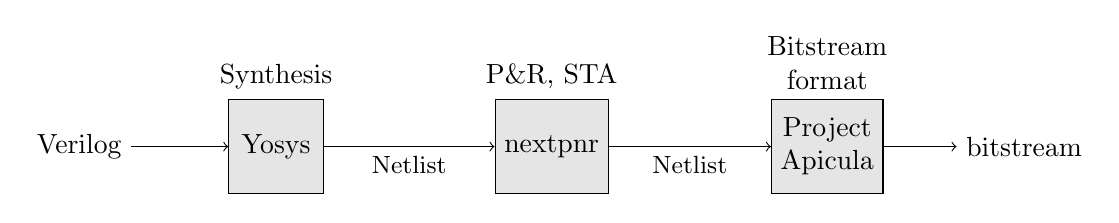
\begin{tikzpicture}[
  block/.style = {
    draw,
    shape=rectangle,
    minimum width=1.2cm,
    minimum height=1.2cm,
    fill=gray!20,
    align=center
  },
  %every path/.style={
  %  very thick,
  %  postaction={
  %    nomorepostaction,
  %    decorate,
  %    decoration={markings,mark=at position 0.5 with {\arrow{>}}}
  %  }
  %}
  %user/.style = {draw, shape=circle, inner sep=0, minimum size=2mm, align=center},
  %arrow/.style = {-Straight Barb},
]
  \node (verilog) {Verilog};
  \node (yosys)[
    right of=verilog,
    label=above:{Synthesis},
    block,
    xshift=15mm
  ] {Yosys};
  \node (nextpnr)[
    right of=yosys,
    %label=above:{P\&R},
    label=above:{\parbox[c]{3.0cm}{\centering P\&R, STA}},
    block,
    xshift=25mm
  ] {nextpnr};
  \node (apicula)[
    right of=nextpnr,
    label=above:{\parbox[c]{3.0cm}{\centering Bitstream\\format}},
    %label=above:{[align=center]Bitstream\\format},
    block,
    xshift=25mm,
    align=center
  ] {Project\\Apicula};
  \node (bitstream)[
    right of=apicula,
    xshift=15mm
  ] {bitstream};

  \draw[->] (verilog) -- (yosys);
  \draw[->] (yosys)   -- (nextpnr) node[below,midway] {\small Netlist};
  \draw[->] (nextpnr) -- (apicula) node[below,midway] {\small Netlist};
  \draw[->] (apicula) -- (bitstream);
\end{tikzpicture}

% \end{document}
